\documentclass[10pt, twocolumn,letterpaper]{article}
%\usepackage[margin=1in]{geometry}
\usepackage{cvpr}
%\usepackage{graphicx}
\usepackage[font=small, labelfont=bf]{caption}
\usepackage{subcaption}
%\usepackage{hyperref}
%\usepackage{xcolor}
%\usepackage{nameref}
%\usepackage{multirow}
%\usepackage{amsmath}
%\usepackage{mathtools}
\usepackage{times}
\usepackage{epsfig}
\usepackage{graphicx}
\usepackage{amsmath}
\usepackage{amssymb}
\usepackage{booktabs}
\usepackage[breaklinks=true,bookmarks=false]{hyperref}
\usepackage[sorting=none, maxcitenames=2]{biblatex}
\addbibresource{bibliography.bib}
\setlength{\parindent}{0pt}

\cvprfinalcopy

% Title Page
\title{Hand-Drawn Graph Recognition\\
	ECE-549 / CS-543\\
	Project Report}
\author{Debopam Sanyal (dsanyal2) \and Neeraj Gangwar (gangwar2) \and Bryan Huang (bryanh2)}
% \date{}


\begin{document}
	\maketitle
	
	\section{Updated Goal}

Our goal remains the same. At the minimum, we want to reproduce graphs from sketches in an online configuration as described in \citeauthor{daly2015hand} \cite{daly2015hand} (we are developing the code from scratch). Our ambitious goal is to be able to implement a successful offline version too.\\

\section{Member Roles}

Neeraj: segmentation, Bryan: classification, Debopam: interpretation and training. All of us will work on integrating the subparts into a whole. We use Github to maintain and share data (\href{https://github.com/neerajgangwar/graph-recognition}{Github Repository}). We meet once a week to discuss updates and issues.

\section{Proposed Approach, Data, Initial Results}

Please see Segmentation, Classification and Domain Interpretation sections for extensive details.


	
	\section{Segmentation}
The first step towards graph recognition is segmentation. This step identifies the segmentation points in the input graph. These points are fed into the recognition task to identify a component. Our implementation is based on the idea presented by \citeauthor{daly2015hand} \cite{daly2015hand} and assumes that the entire component is drawn in one stroke. However, drawing multiple components in the same stroke is acceptable for our implementation.\\

The segmentation points identify the transition from one component to the next. These are referred to as true segmentation points.  However, there are certain challenges in the segmentation task. These challenges arise from the fact that there might be additional points in a component with similar geometric properties as true segmentation points. This is shown in Figure \ref{fig:seg_false_neg}. The challenges can be divided into two buckets: false positives and false negatives. The points that are incorrectly identified as segmentation points contribute to false positives. These cases are less severe as they can be handled in the classification step. The points that are true segmentation points but are missed by the segmentation algorithm are false negatives. These cases are more severe as we cannot recover from these errors. The goal of the segmentation algorithm would be to minimize false positives while ensuring that there are no false negatives.\\

\begin{figure}
	\centering
	\begin{subfigure}{0.3\textwidth}
		\centering
		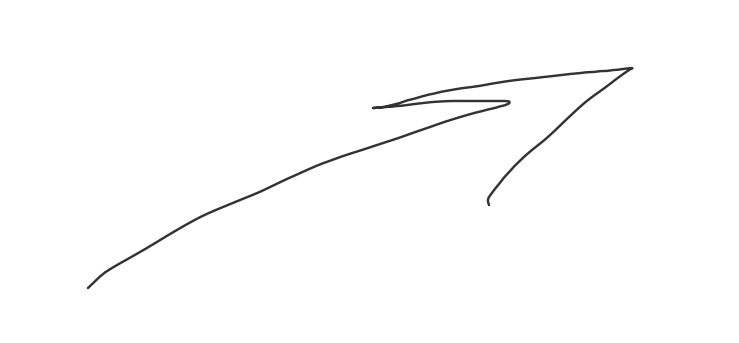
\includegraphics[scale=0.2]{./img/seg_orig.jpg}
	\end{subfigure}
	\begin{subfigure}{0.3\textwidth}
		\centering
		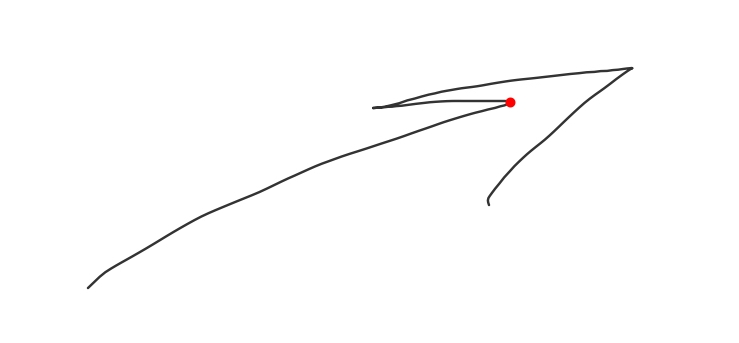
\includegraphics[scale=0.2]{./img/seg_true_seg.jpg}
	\end{subfigure}
	\begin{subfigure}{0.3\textwidth}j
		\centering
		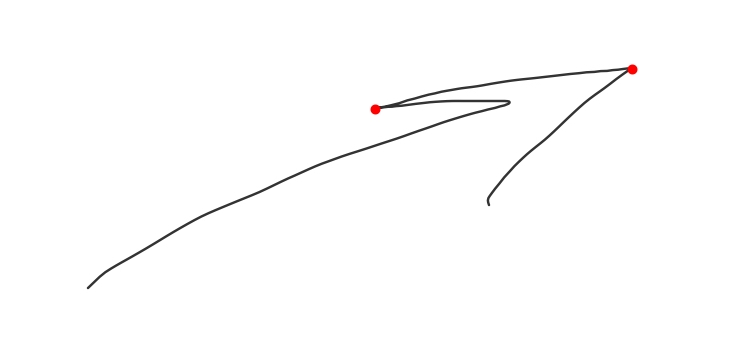
\includegraphics[scale=0.2]{./img/seg_false_seg.jpg}
	\end{subfigure}
	\caption{\textit{left} a line and arrow head drawn in one stroke, \textit{middle} true segmentation point, \textit{right} additional points with similar properties as true segmentation points}
	\label{fig:seg_false_neg}
\end{figure}

\subsection{Algorithm}
The algorithm to identify segmentation points is based on the observation that there are abrupt changes in curvature at these points. This is based on the properties of transition that can occur in the three types of graph components. This is shown in figure \ref{fig:seg_curvature}.\\

Before the curvature calculation, some pre-processing of input data is required. We use iPyCanvas \cite{ipycanvas} to capture the coordinates of the drawn components. The number of coordinates captured depends on the drawing speed. If the drawing speed is higher in certain regions, the number of points captured will be higher in those region. This count is normalized by considering the distance between two points. If the Euclidean distance between two consecutive points, $P_i$ and $P_{i+1}$, is less than a threshold, $d_t$, we drop $P_{i+1}$. Here, $d_t$ is a hyperparameter which needs to be trained based on the input data. For our usecase, $d_t = 1$ works well.\\

The curvature of a point $P_i$ is computed by calculating the angles between vectors formed by joining $P_{i-s}$ and $P_i$ and $P_i$ and $P_{i+s}$. $s$ is the second hyperparameters. For our usecase, we have kept $s=3$ based on experiments.

\begin{equation}
	C_s(P_i) = \arccos \left(  \frac{\overrightarrow{P_{i-s} P_i} \cdot \overrightarrow{P_i P_{i+s}}}{ \Vert \overrightarrow{P_{i-s} P_i}  \Vert \; \Vert \overrightarrow{P_i P_{i+s}} \Vert  } \right) 
\end{equation} 

Once the curvature is computed for all captured points, we compute the abnormality. This metric is used in identifying the abrupt and significant changes in the curvature. The abnormality of a point $P_i$ is defined by how the curvature at that point differs from the average curvature of the surrounding points.
\begin{equation}
	A_{s,w}(P_i) = C_s(P_i) - \frac{\sum_{j=a}^{i-1} C_s(P_j) + \sum_{j=i+1}^{b} C_s(P_j)}{b - a}
\end{equation}
where $a = max(1, i-w)$ and $b = min(n, i+w)$.\\

$w$ is the third hyperparameter. For our usecase, we use $w=5$ based on our experiments. Next, we need to find ranges of points where $k A_{s, w}(P_i) > 1$ and select the point with maximum abnormality in each range as the segmentation point. The multiplication factor $k$ is the fourth hyperparameter.\\

\begin{figure}
	\centering
	\begin{subfigure}{0.9\textwidth}
		\centering
		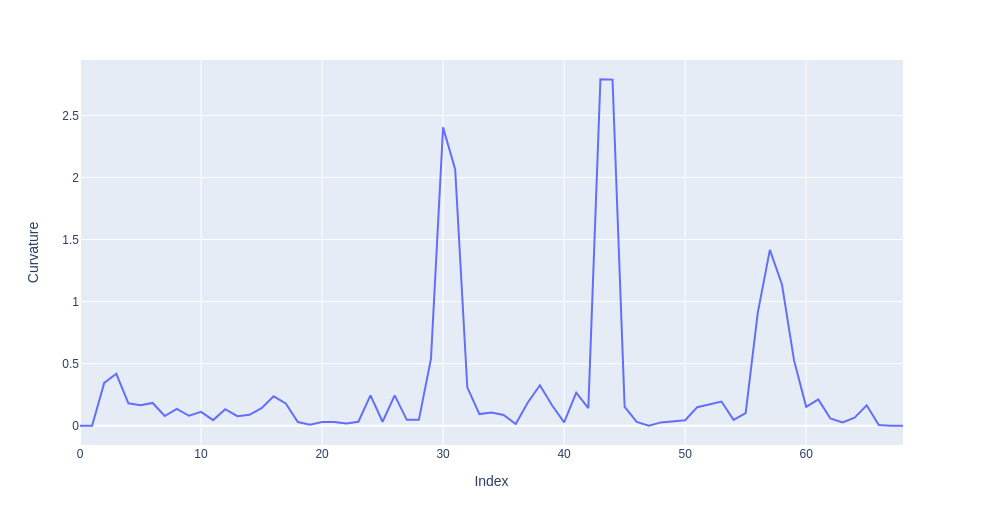
\includegraphics[scale=0.5]{./img/seg_curvature_plot}
	\end{subfigure}
	\caption{Curvature plot for the components shown in figure \ref{fig:seg_false_neg}. The peaks represent the segmentation points.}
	\label{fig:seg_curvature}
\end{figure}

\subsection{Experiments}
To test the segmentation algorithm, we drew some components and shapes manually on iPyCanvas and validated the results. These are shown in figure \ref{fig:seg_results}.
\begin{figure}
	\centering
	\begin{subfigure}{0.8\textwidth}
		\centering
		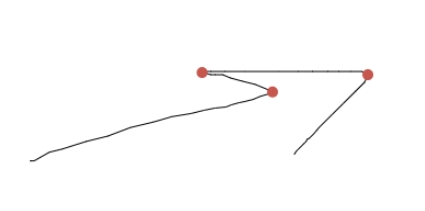
\includegraphics[scale=0.6]{./img/seg_results_arrow.jpg}
	\end{subfigure}
	\begin{subfigure}{0.8\textwidth}
		\centering
		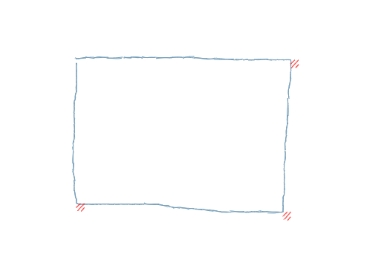
\includegraphics[scale=0.6]{./img/seg_results_rect.jpg}
	\end{subfigure}
	\begin{subfigure}{0.8\textwidth}
		\centering
		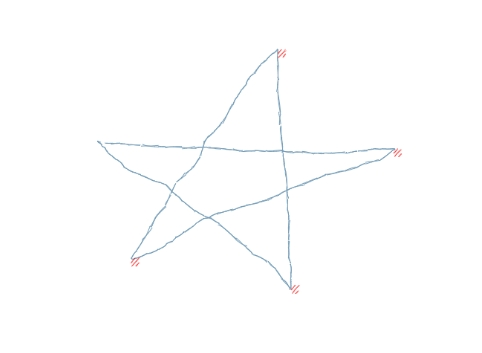
\includegraphics[scale=0.6]{./img/seg_results_pentagram.jpg}
	\end{subfigure}
	\caption{Detected segmentation points (highlighted in red).}
	\label{fig:seg_results}
\end{figure}

\subsection{Future Work}
The immediate next step is to integrate the segmentation module with the classification module and fine tune the four hyperparameters discussed in this section. In addition, we will work on extending the algorithm to support offline graph recognition.
	
	\section{Classification}
\label{sec:classification}

After segmentation is completed, we run classification on each segment. This is to determine the probability that a given segment is one of four types - vertex, self-loop, edge, or arrow. These probabilities are used in domain interpretation step to reconstruct the original graph. 

\subsection{Original Algorithm}

The first version of classification we implemented was a recreation of the original paper. In order to determine the segment's probability distribution, we find five parameters. These parameters were chosen by \citeauthor{daly2015hand} \cite{daly2015hand}, based on the alpha shape and convex hull of the segment. \\ 

To compute the alpha shape and convex hull, we use the Alpha Shape Toolbox library \cite{alphashapetoolbox}, as well as SciPy's ConvexHull implementation \cite{scipy}. These libraries provide tools to easily find the area, perimeter, and points of these shapes. \\

\subsubsection{Circumscribed circle}

The first parameter is used to distinguish vertices and loops from other segments. This parameter $x_1$ is computed as \\

\begin{equation}
	x_1 = \frac{\text{Area of Convex Hull}}{\text{Area of circumscribed circle of Convex Hull}}
\end{equation} \\

The convex hull is not necessarily cyclic, so we define the circumscribed circle as a circle with diameter equal to the distance between the two farthest points in the convex hull. \\

\subsubsection{Inscribed triangle}

The second parameter is used to distinguish arrows. This parameter $x_2$ is computed as \\

\begin{equation}
	x_2 = \frac{\text{Area of largest inner triangle with angles over 20\textdegree}}{\text{Area of Convex Hull}}
\end{equation} \\

We use the method by \citeauthor{largesttriangle} \cite{largesttriangle} to find the area of the largest inner triangle.

\subsubsection{Alpha shape ratio}

The third parameter is used to distinguish line segments. This parameter $x_3$ is computed as \\

\begin{equation}
	x_3 = \frac{\text{Perimeter of alpha shape with $\alpha$ = 25}}{500 \cdot \text{Area of alpha shape with $\alpha$ = 25}}
\end{equation} \\

\subsubsection{Perimeter}

The fourth parameter is used to distinguish vertices and arrows from other segments. This parameter $x_4$ is computed as \\

\begin{equation}
	x_4 = \frac{\text{Perimeter of Convex Hull}}{\text{500}}
\end{equation} \\

\subsubsection{Disjoint shapes}

The final parameter disqualifies any strokes that are not properly segmented. This parameter $x_5$ is computed as

\begin{equation}
	x_5 = \; \parbox{14em}{Number of disjoint regions in alpha shape over 50 pixels apart} - 1
\end{equation}

The weights applied to each parameter reflect traits held by classes of stroke. For example, vertices and self-loops are almost circular, so they assign high positive weight to the circumscribed circle parameter. For testing purposes, we use the original weights trained by \citeauthor{daly2015hand} \cite{daly2015hand}. Notably, the weight for parameter $x_5$ is not trained, and instead set to always be -1000, to minimize the probability distribution of any shape with multiple disjoint regions.

\subsection{Offline Implementation}

Classification, unlike segmentation and domain interpretation, can be accomplished without needing the chronological order of drawn points. As long as the collection of points is present, features can be extracted without any significant difference in effectiveness. Within our implementation, the only feature computed with exponential complexity is the circumscribed circle, and that feature can be computed in polynomial time through rotating calipers. \\

There is the consideration of the input points being too granular. The original paper handles this by removing any line segments greater than a given distance. This implementation requires chronological order of points, but we can accomplish a similar level of granularity through downsampling the input pixels.

\subsection{CNN Approach}
While classification does not need significant improvements to be effective both online and offline, we explored training a CNN as another method for classification. \citeauthor{daly2015hand}'s implementation of classification was trained on manually chosen features, so we attempted to see how features extracted by CNN would complete the same problem.\\

Creating and labelling data would take a significant amount of time for an exploration, and there are no public data sets for this particular problem that we could find. Because the classes of graph components are so simple in shape, we can use a data set like MNIST, with only a few changes. MNIST is a very basic and commonly used data set, so almost any network can easily achieve a very high accuracy. However, high accuracy on the MNIST test set does not translate to high accuracy with our task. \\

This method cannot differentiate self-loops and vertices as effectively as the original paper. For this reason we change number of classes to 3 rather than 4, combining vertices and self-loops into one class. The primary difference between the two classes is the perimeter of the stroke. The original implementation is able to differentiate by using perimeter as a feature. We would need to make the network scale-aware, and further preprocess the data set. \\

Another issue with this method is that domain interpretation requires additional information not used in classification that the CNN cannot extract. The hand-picked features for classification are similar enough to the features needed for domain interpretation that it is efficient to compute simultaneously, which cannot be done by the CNN. \\

Line thickness also negatively affects this method. In the online case, the original method does not need image data and extracts points through the canvas. In the offline case, the original method can use erosion to reduce a stroke to a list of relevant points. However, in the CNN method, the MNIST dataset contains training images with particular line widths. Assuming that a drawn graph has consistent line width throughout, after resizing strokes with different sizes, the resulting CNN inputs would have different line widths. In our demonstration notebook, we use a fixed canvas size and line width, but in experiments, we found that too small of a line width would make classification incorrect. \\

Due to all of the above considerations, we found that stroke classification is better suited to using hand-picked geometric features than recognition through CNN.

\subsubsection{Dataset}

We used a modified version of the MNIST dataset. All entries labelled with a digit other than 0, 1, and 7 were removed from the dataset. The resulting dataset contained 24,888 training images and 4,175 test images. We randomly rotate the training input within a range of 360 degrees, in order to train for all possible orientations.

\subsection{Experiments}
Similarly to the segmentation algorithm, we tested classification by drawing single strokes on the iPyCanvas. One example is shown in Figure \ref{fig:classification_example}.

For the CNN method, we used the test dataset described above.

\begin{figure}
	\centering
	\begin{subfigure}{0.45\textwidth}
		\centering
		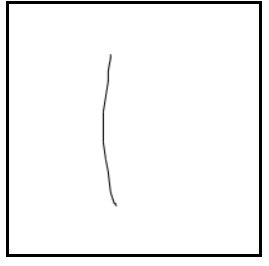
\includegraphics[scale=0.5]{./img/classificationexample}
	\end{subfigure}
	\caption{Example segment. $p_{vertex} = 0.0000076\text{, }   p_{arrow} = 0.256\text{, } p_{edge} = 0.996\text{, }  p_{loop} = 0.000086$}
	\label{fig:classification_example}
\end{figure}

%\subsection{Future Work}
%
%Our future work is to connect the probability distributions computed in this step to the domain interpretation step. Certain classes tend to have similar probabilities, for example, vertices and self-loops are difficult to differentiate. These are typically differentiated in domain interpretation rather than classification. \\
%
%In addition, we may need to further test these implementations on more data, or train more on our own data so that our weights better reflect our specific implementations.


	
	\section{Domain Interpretation}
\label{sec:interpretation}

After we compute the probabilities from the classification section, we need to produce a final interpretation of the graph in terms of edges, vertices, arrows, self-loops, connections between edges and vertices and connections between arrows and edges. To do this we cannot use the trivial method of partitioning the graph into segments (from our segmentation step) and  simply solving for the partition that produces the largest sum of classification probabilities (from the classification step). This is mainly because there is significant interaction between components of a graph. The design that we follow rests on the idea that the connections between the components influence the selection of the best interpretation.\\

We found it useful to rank candidate graphs by scores that are formed from a range of metrics like classifier probabilities (g(p)), total number of components (C(p)), number of connections (D(p)) and number of missing connections (M(p)). Thus, the score is simply: $V_{A,B,C}(p) = g(p) + A.C(p) + B.D(p) + C.M(p)$ where $g(p) = \sum_{(a_i,b_i,c_i) \in p}f(a_i+b_i+t_i)$. The function f is determined by the  classification probabilities. The score however is 0 when any component in p has a probability less 0.2. To properly asses the connections, we had to establish a set of machine specifications for our components where we could find the distances, say, between an edge and vertex or an edge an arrow.\\

\subsection{Algorithms}

The algorithm section can be divided into 2 parts: 1) domain interpretation and 2) training the score parameters.\\

\subsubsection{Connections}

A vertex-edge connection is tested for every vertex and edge pair. We can use the center and radius of the vertex to find the distance from the endpoints of the edge as edges are given as a set of target points that represent a smooth line. Computing the Euclidean distance between the center and each of the two endpoints of the edges gives us an idea of whether the connection is plausible. Of course, we have to subtract the radius of the circle itself and threshold the resulting distance to discard the large distance values. We maintain a score q for each edge end point that is initialized to infinity and updated if and only if a new vertex is found for the end point such that it's distance falls below the threshold and it is less than the previous q (negative values are clipped to 0).\\

The arrow-edge connection algorithm is more complex because it involve triangles (machine specification for arrows) and lines (edges) that have to intersect one of the sides of the triangle. Again, connection is tested for every arrow and edge pair (from the endpoints of the edge). Here, we first extend the edge sequence by adding a target point before the end point such that smoothness is still maintained (use the slope for this). The distance between the new and the old point is $\gamma$ . Now, we test for the segment between each consecutive pair of the extended edge. If the segment intersects with a side of the triangle, then two conditions have to satisfied. The first is that the distance between the endpoint and the point of intersection has to be under the threshold or the distance between the endpoint and the point opposite to the intersection side of the triangle has to be under the threshold. The second condition is valid only for arrows that were initially two-sided. It states that the side involved in the intersection is the same as the one that was initially non-represented by the user's drawing.\\

\subsubsection{Training the parameters}

Training is done by post-processing the sketches of users. Since we are implementing the online method now, our recognition is triggered a fixed time after the user stops sketching. We do not want the already graph to change. Hence, the "locked-in" portion of the graph doesn't change here. New connections are made between the newly drawn components and the locked in components by a recognizer. The recognizer maintains a sequence of added strokes and the corresponding sub-graphs. For every pair, we select the most promising candidate graph according to our scores. However, if an isomorph exists, we select the isomorph as the representation of the intermediate subgraph. If there exists no isomorphism then we penalize all the remaining pairs of new strokes and subgraphs.\\

\section{Future Work}
For segmentation, the immediate next step is to integrate the segmentation module with the classification module and fine tune the four hyperparameters discussed in this section. In addition, we will work on extending the algorithm to support offline graph recognition.\\


For classification, our future work is to connect the probability distributions computed in this step to the domain interpretation step. Certain classes tend to have similar probabilities, for example, vertices and self-loops are difficult to differentiate. These are typically differentiated in domain interpretation rather than classification. In addition, we may need to further test these implementations on more data, or train more on our own data so that our weights better reflect our specific implementations.\\

For domain interpretation, we are still in the process of developing the training algorithm. We are currently working on how to decide on a list of candidate graphs. One option is to use close component classification probabilities to create a set of plausible graphs. Our algorithm to find the isomorphism and line-triangle intersection still need testing. The other functions have been tested on dummy probabilities. However, we still are yet to integrate the segmentation and classification sections to this section, which is why this section has not yet been tested on real examples yet.\\

After successfully completing the online method, we will work on the offline method. There are some fundamentally different aspects to the offline method like the recognizer will only act on the graph after completion and connections do not have to maintained to a locked-in graph. We aim to have an effective offline interpretation as our ambitious goal.\\
	
	\section{Conclusion and Future Work}
	In this project, we worked on the online graph recognition problem. For offline recognition, we tried to use the same pipeline by converting an offline graph to a sequence of coordinates. But this approach was not successful as the current pipeline heavily relies on the ordering of the coordinates. The offline recognition problem can be modeled as a learning problem and deep learning approaches can be used to solve it.\\
	
	The segmentation algorithms discussed in this report heavily rely of hyperparameter tuning. The values of these parameters can vary from person-to-person. Rather than finding the parameter values that work for everyone, we can tune these parameter for an individual by taking feedback from the user. The speed-based segmentation can be explored further. To reduce the false-positives, an abnormality computation step similar to the curvature-based segmentation can be added to overcome the noise.\\
	
	For classification, we found that it was a task well-suited to multiple pipeline configurations, only needing to adjust the input format. The geometric feature approach described in the original paper was the most effective. The problem is simple enough that attempting convolutional methods introduces significant complexity for minimal increase in efficacy.\\
    
    Classification is simple enough not to need an approach more complex than the features discussed here, but it is closely related to segmentation. Future work could include an object detection method to perform both tasks simultaneously.\\
    
    In the current pipeline, the output needs to be evaluated by inspecting probabilities and costs.  It can be replaced with a user interface to visualize the output. It is a required feature for the end-user and will significantly reduce the time to analyze the performance of this pipeline.
	
	\section{Member Roles}
	Neeraj: segmentation, Bryan: classification, Debopam: interpretation and training. All of us worked on integrating the subparts into a whole. We used Github to maintain and share data (\href{https://github.com/neerajgangwar/graph-recognition}{Github Repository}). We met once a week to discuss updates and issues.
	
	\printbibliography[title=References]
	
\end{document}
